\documentclass[11pt]{article}

\usepackage[margin=1in]{geometry}
\usepackage[T1]{fontenc}
\usepackage{lmodern}
\usepackage{amsmath, amssymb}
\usepackage{setspace}
\usepackage[most]{tcolorbox}
\usepackage{xcolor}
\usepackage{fancyhdr}
\usepackage{listings}
\usepackage{upquote}
\usepackage{adjustbox}

\pagestyle{fancy}
\fancyhf{}
\setlength{\headheight}{52pt}
\renewcommand{\headrulewidth}{0pt}

\tcbset{enhanced,boxrule=0pt,frame hidden,breakable}

\newcommand{\Course}{Math 4610 Spring 2026}
\newcommand{\Instructor}{Discussion 7}
\newcommand{\AssignmentType}{Discussion}
\newcommand{\AssignmentNumber}{7}
\newcommand{\Contributors}{Stephen Marks}

\fancyhead[L]{\Course\\ \Instructor}
\fancyhead[R]{\Contributors}

\newcommand{\ProblemDivider}[1]{%
  \vspace{1.0em}
  \noindent\textbf{#1}\par
  \vspace{0.35em}
}

\definecolor{exerciseGray}{gray}{0.96}
\definecolor{exerciseGrayFrame}{gray}{0.45}

\newtcolorbox{problemBox}{
  colback=exerciseGray,
  colframe=exerciseGrayFrame,
  arc=2mm,
  left=8pt,right=8pt,top=8pt,bottom=8pt
}

\newtcolorbox{solutionBox}{
  colback=white,
  colframe=white,
  arc=0mm,
  left=0pt,right=0pt,top=0pt,bottom=0pt
}

\newtcolorbox{codeBox}{
  colback=gray!6,
  colframe=gray!55,
  boxrule=0.6pt,
  arc=1.5mm,
  left=6pt,right=6pt,top=6pt,bottom=6pt,
  breakable
}

\newcommand{\ProblemAnnounce}{\noindent}
\newcommand{\SolutionAnnounce}{\noindent\textbf{Solution.}\par\medskip}
\newcommand{\R}{\mathbb{R}}
\newcommand{\Exercise}[1]{\textbf{Exercise~#1.}\;}

\lstset{
  basicstyle=\ttfamily\small,
  columns=fullflexible,
  keepspaces=true,
  showstringspaces=false,
  language=Python
}

\begin{document}

\begin{center}
  {\Large \textbf{\AssignmentType~\AssignmentNumber}}
\end{center}
\vspace{0.75em}

\ProblemDivider{1}
\begin{problemBox}
\ProblemAnnounce
Does $f(t)=\sin(\pi t)$ belong to $P_6(\R)$? Why?
\end{problemBox}

\begin{solutionBox}
\SolutionAnnounce
\doublespacing
No. The space $P_6(\R)$ consists of polynomials of degree at most $6$, and $\sin(\pi t)$ is not a polynomial. Therefore $f \notin P_6(\R)$.
\end{solutionBox}

\ProblemDivider{2}
\begin{problemBox}
\ProblemAnnounce
Consider the function $F:P_6(\R)\to\R$ defined by
\[
F(p):=\int_{-1}^{1} p(t)f(t)\,dt.
\]
Prove that $F$ is a functional on the space $P_6(\R)$.
\end{problemBox}

\begin{solutionBox}
\SolutionAnnounce
\doublespacing
To show that $F$ is a functional, it suffices to show that $F$ is linear.

Let $p,q\in P_6(\R)$ and $a\in\R$. Then
\[
F(p+q)=\int_{-1}^{1} (p(t)+q(t))f(t)\,dt
=\int_{-1}^{1} p(t)f(t)\,dt+\int_{-1}^{1} q(t)f(t)\,dt
=F(p)+F(q),
\]
and
\[
F(ap)=\int_{-1}^{1} a\,p(t)f(t)\,dt
=a\int_{-1}^{1} p(t)f(t)\,dt
=aF(p).
\]
Thus $F$ is a linear map from $P_6(\R)$ to $\R$, so $F$ is a functional.
\end{solutionBox}

\newpage
\ProblemDivider{3}
\begin{problemBox}
\ProblemAnnounce
By the Riesz Representation Theorem, there should be $u\in P_6(\R)$ such that
\[
F(p)=\langle p,u\rangle.
\]
Find such a $u$.
\end{problemBox}

\begin{solutionBox}
\SolutionAnnounce
\doublespacing
We need to show $u\in P_6(\R)$ such that
\[
\langle p,u\rangle=\int_{-1}^{1} p(t)u(t)\,dt=\int_{-1}^{1} p(t)\sin(\pi t)\,dt
\quad\text{for all } p\in P_6(\R).
\]
Thus $u$ is the orthogonal projection of $\sin(\pi t)$ onto $P_6(\R)$.

Since $\sin(\pi t)$ is odd, only the odd basis vectors contribute, so 
\[
u(t)=c_1 t+c_3 t^3+c_5 t^5.
\]
Then 
\[
\langle t^k,u\rangle=\langle t^k,\sin(\pi t)\rangle
\quad\text{for } k=1,3,5.
\]
This gives the linear system
\[
\begin{bmatrix}
\frac23 & \frac25 & \frac27\\
\frac25 & \frac27 & \frac29\\
\frac27 & \frac29 & \frac{2}{11}
\end{bmatrix}
\begin{bmatrix}
c_1\\ c_3\\ c_5
\end{bmatrix}
=
\begin{bmatrix}
\frac{2}{\pi}\\[2mm]
\frac{2}{\pi}-\frac{12}{\pi^3}\\[2mm]
\frac{2}{\pi}-\frac{40}{\pi^3}+\frac{240}{\pi^5}
\end{bmatrix}.
\]
Solving results in
\[
c_1=\frac{105\bigl(\pi^4-153\pi^2+1485\bigr)}{8\pi^5},
\qquad
c_3=\frac{315\bigl(125\pi^2-\pi^4-1155\bigr)}{4\pi^5},
\qquad
c_5=\frac{693\bigl(\pi^4-105\pi^2+945\bigr)}{8\pi^5}.
\]
Therefore
\[
\boxed{
u(t)=\frac{105(\pi^4-153\pi^2+1485)}{8\pi^5}t
+\frac{315(125\pi^2-\pi^4-1155)}{4\pi^5}t^3
+\frac{693(\pi^4-105\pi^2+945)}{8\pi^5}t^5.}
\]
Numerically,
\[
\boxed{u(t)\approx 3.1034604279\,t-4.8143883186\,t^3+1.7269051843\,t^5.}
\]
So this polynomial is the Riesz representative of $F$ in $P_6(\R)$.

\medskip
This solution is verified by the following sage script:

\begin{codeBox}
  \begin{lstlisting}[language=Python]
var('t')
f = sin(pi*t)

# inner product on P6(R)
def ip(v, u):
    return integrate(v*u, t, -1, 1)

# odd basis because sin(pi*t) is odd
B = [t, t^3, t^5]

A = matrix(SR, [[ip(B[j], B[i]) for j in range(3)] for i in range(3)])
b = vector(SR, [ip(f, B[i]) for i in range(3)])
c = A.solve_right(b)

u = sum(c[i]*B[i] for i in range(3)).full_simplify()
print(u)
\end{lstlisting}
\end{codeBox}
This script outputs:
\begin{codeBox}
\begin{lstlisting}[breaklines=true, breakatwhitespace=true]
u(t) = 21/8*(33*(pi^4 - 105*pi^2 + 945)*t^5 - 30*(pi^4 - 125*pi^2 + 1155)*t^3 + 5*(pi^4 - 153*pi^2 + 1485)*t)/pi^5
\end{lstlisting}
\end{codeBox}
\end{solutionBox}
Which coincides with our findings.

\newpage
\ProblemDivider{4}
\begin{problemBox}
\ProblemAnnounce
Graph $f(t)=\sin(\pi t)$ together with $u(t)$ on the interval $[-1,1]$. What do you notice?
\end{problemBox}

\begin{figure}[]
    \centering
    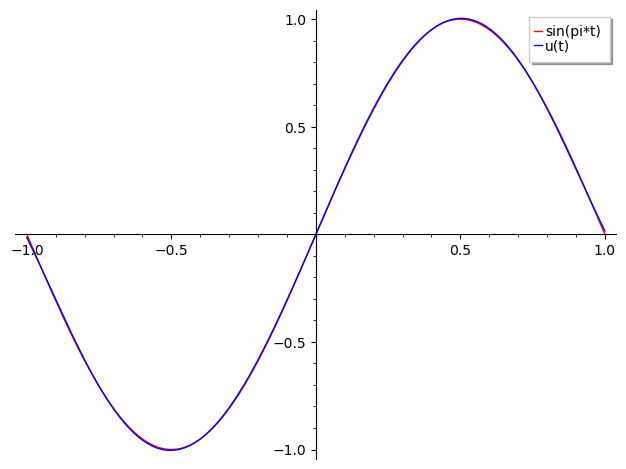
\includegraphics[width=0.55\textwidth]{img/disc_7_plot.png}
    \caption{}
\end{figure}

\begin{solutionBox}
\SolutionAnnounce
\doublespacing
The graph of $u(t)$ follows $\sin(\pi t)$ very closely on $[-1,1]$. Both are odd functions, both pass through $(0,0)$, and the polynomial $u$ has the same overall shape as $\sin(\pi t)$. So $u$ is the best approximation to $\sin(\pi t)$ coming from the subspace $P_6(\R)$ with respect to this inner product. \textit{See Figure 1}
\end{solutionBox}

\end{document}
